\chapter{Coordinates}
\label{s:coords}

\begin{figure}[!hb]
  \centering
  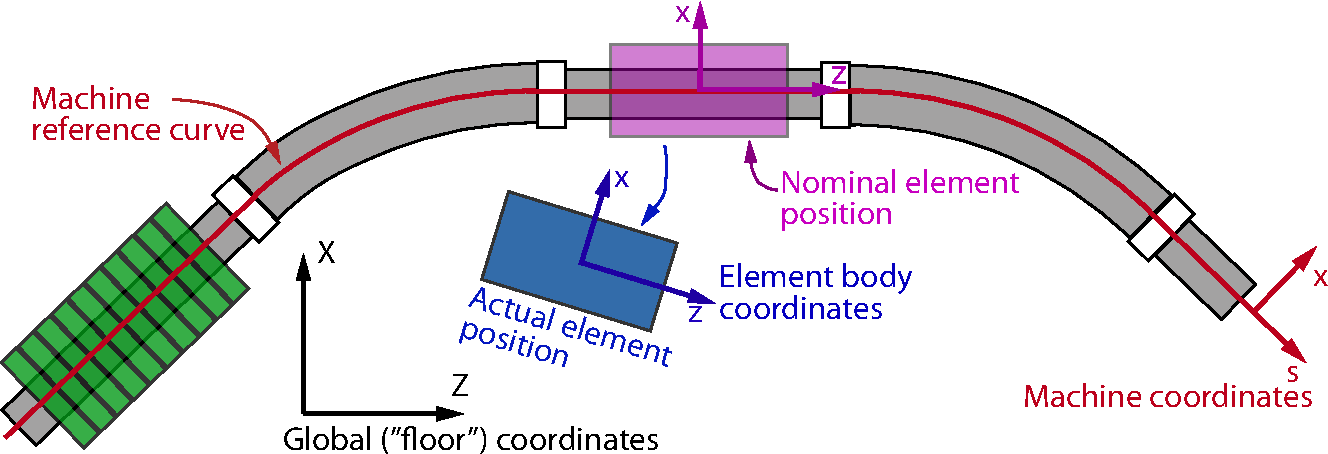
\includegraphics[width=5.0in]{coordinates.pdf}
  \caption[The three coordinate system used by \accellat.]
{The \vn{floor} coordinate system
is independent of the accelerator.  The \vn{branch} curvilinear coordinate system follows the bends
of the accelerator. The \vn{branch reference curve} is the $x = y = 0$ curve of the curvilinear coordinate
system. Each lattice element has \vn{element body} coordinates which, if the element has no
alignment shifts (not ``misaligned''), is the same as the \vn{branch} coordinates.}
  \label{f:coords}
\end{figure}

%---------------------------------------------------------------------------------------------------
\section{Coordinate Systems}
\label{s:coords}
\vspace*{-0.1in}

\accellat uses three coordinate systems as illustrated in \fig{f:coords}. First, the \vn{floor}
coordinates are coordinates independent of the accelerator. The position of the accelerator 
itself as well as external objects like the building the accelerator is in  may be described 
using \vn{floor} coordinates.

It is inconvenient to describe the position lattice elements and the position of a 
particle beam using the \vn{floor} coordinate system so, for each tracking lattice branch,
a ``\vn{branch}'' coordinate system is used (\sref{s:branch.coords}). This curvilinear coordinate
system defines the nominal position of the lattice elements. The relationship between the
\vn{branch} and \vn{floor} coordinate systems is described in \sref{s:floor}. Non-tracking branches
do not have an associated branch coordinate system.

The \vn{branch reference curve} is the $x = y = 0$ curve of the curvilinear coordinate
system. The branch reference curve does not have to be continuous. A non-continuous
reference curve is used, for example, to connect branches together. 

The ``nominal'' position of a lattice element is the position of the element without any
position and orientation shifts (\sref{s:align.g}) 
which are sometimes referred to as ``misalignments''. 
Each lattice element has ``\vn{element body}'' (or just ``\vn{body}'') 
coordinates which are attached to the physical element and the electric and magnetic
fields of an element are described with respect to \vn{body} coordinates.  
If an element has no
alignment shifts, the \vn{body} coordinates of the element are aligned with the 
\vn{branch} coordinates.
The transformation between \vn{branch} and \vn{body} coordinates is given in
\sref{s:lab.body.transform}.

%--------------------------------------

  \begin{figure}[tb]
  \centering
  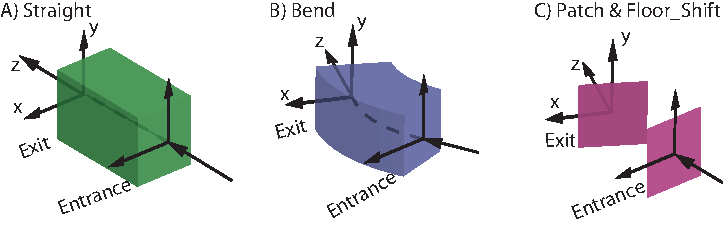
\includegraphics[width=5in]{ele-coord-frame.pdf}
\caption[Lattice elements as LEGO blocks.]{Lattice elements can be imagined as ``LEGO blocks'' which
fit together to form the branch coordinate system. How elements
join together is determined in part by their entrance and exit coordinate frames. A) For
straight line elements the entrance and exit frames are colinear. B) For bends elements, the two
frames are rotated with respect to each other. C) For \vn{Patch} and \vn{floor_shift} elements the
exit frame may be arbitrarily positioned with respect to the entrance frame.}
  \label{f:ele.coord.frame}
  \end{figure}

%--------------------------------------

%---------------------------------------------------------------------------------------------------
\section{Element Entrance and Exit Coordinates}
\label{s:ent.exi}

As discussed in the next section, the branch coordinate system is constructed starting with the first
element in a lattice tracking branch and then building up the coordinate system element-by-element.
All elements in a tracking branch have an ``\vn{entrance}'' and an ``\vn{exit}'' coordinate frame as
illustrated in \fig{f:ele.coord.frame}
These coordinate frames are attached to the element and are part of the \vn{element body coordinates}. 
An exception occurs if there are \vn{Fiducial} elements (\sref[s:fiducial}) in a branch. 
\vn{Fiducial} elements only have a single coordinate frame that is tied to global coordinates 
and construction of the branch coordinate system starts at this coordinate system. 
See \sref{s:fiducial} for more details.
Note that \vn{Girder} elements (\sref{s:girder}) also only have a single coordinate frame.

Most element types have a ``straight'' geometry as shown in
\fig{f:ele.coord.frame}A. That is, the reference curve through the element is a straight line
segment with the $x$ and $y$ axes always pointing in the same direction. For a \vn{Bend} element
(\sref{s:bend}), the reference curve is a segment of a circular arc as shown in
\fig{f:ele.coord.frame}B. With the \vn{ref_tilt} parameter of a bend set to zero, the rotation axis
between the entrance and exit frames is parallel to the $y$-axis (\sref{s:floor}). 
For \vn{Patch} (\sref{s:patch}) and \vn{floor_shift} (\sref{s:floorshift})
elements (\fig{f:ele.coord.frame}C), the exit face can be
arbitrarily oriented with respect to the entrance end. 
For \vn{FloorShift} elements the interior reference curve between the
entrance and exit faces is not defined. For the \vn{Patch} element, the interior reference curve 
is dependent upon certain \vn{Patch} element parameter settings (\sref{s:patch}).

%---------------------------------------------------------------------------------------------------
\section{Branch Coordinates Construction}
\label{s:ref.construct}

%-----------------------------------------------------------------------------
\begin{figure}[tb]
  \centering
  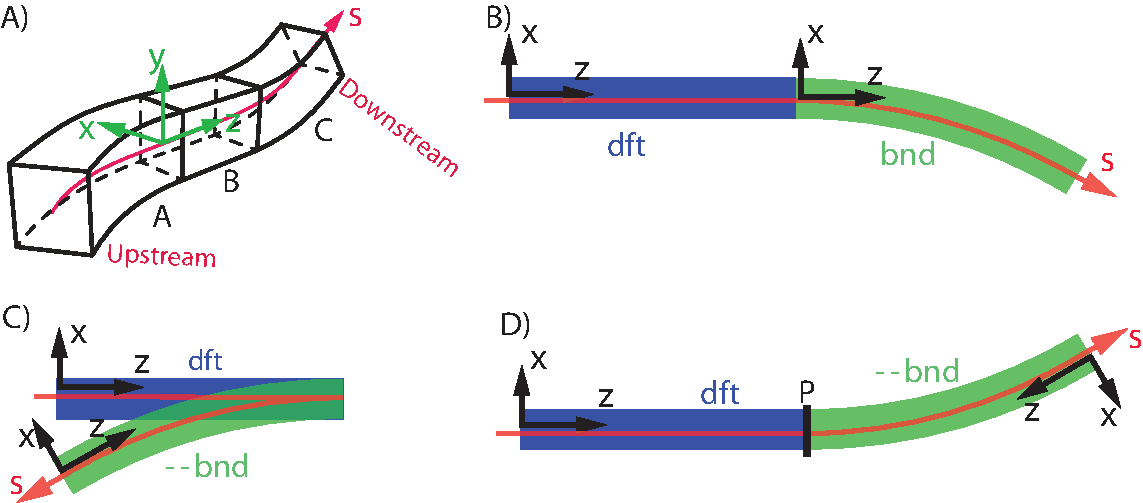
\includegraphics[width=5in]{patch-between.pdf}
  \caption[Branch coordinates construction.]{A) The branch coordinates are constructed by
connecting the \vn{downstream} reference frame of one element with the \vn{upstream} reference frame
of the next element in the branch. Coordinates shown is for the mating of element \vn{A} to element
{B}.  B) Example with drift element \vn{dft} followed by a bend \vn{bnd}. Both elements are
unreversed. C) Similar to (B) but in this case element \vn{bnd} is reversed.  D) Similar to (C) but
in this case a reflection patch has been added in between \vn{dft} and \vn{bnd}.  In (B), (C), and
(D) the $(x,z)$ coordinates are drawn at the \vn{entrance} end of the elements. The $y$ coordinate
is always out of the page.}
  \label{f:patch.between}
\end{figure}
%-----------------------------------------------------------------------------

Assuming for the moment that there are no \vn{Fiducial} elements present, the construction of the
branch coordinate system starts at the \vn{BeginningEle} element (\sref{s:begin.ele}) at the start of a
branch. If the branch is a \vn{root} branch (\sref{s:lattice.def}), The orientation of the beginning
element within the floor coordinate system (\sref{s:coords}) can be fixed by setting 
\vn{OrientationParams parameters} (\sref{s:orientationition.g}) in the \vn{BeginningEle} element.
If the branch is not a \vn{root} branch, the position
of the beginning element is determined by the position of the \vn{Fork} element
from which the branch forks from. The default value of $s$ at the \vn{BeginningEle} element is zero
for both root and non-root branches.

Once the beginning element in a branch is positioned, succeeding elements are concatenated together
to form the branch coordinate system. All elements have an ``\vn{upstream}'' and a ``\vn{downstream}''
end as shown in \fig{f:patch.between}A. The \vn{downstream} end of an element is always farther (at
greater $s$) from the beginning element than the \vn{upstream} end of the element. Normally,
particles will travel
in the $+s$ direction, so particles will enter an element at the upstream end and exit at the
downstream end.

If there are \vn{Fiducial} elements, the branch coordinates are constructed beginning at these
elements working both forwards and backwards along the branch. 
If there are multiple \vn{Fiducial} elements in a branch, there must be flexible \vn{Patch}
elements (\sref{s:patch}) between them.

If an element is not reversed (\sref{s:ele.reverse}),
the element's \vn{upstream} end is the same as the element's \vn{entrance} end 
(\fig{f:ele.coord.frame}) and the
\vn{downstream} end is the same as the element's \vn{exit} end and
vice versa if the element is reversed, 
That is, for a reversed element, particles 
traveling downstream will
enter at the element's \vn{exit} end and will exit at the \vn{entrance} end.

The procedure to connect elements together to form the branch coordinates is to ignore 
alignment shifts and mate the
downstream reference frame of the element with the upstream reference frame of the next element in
the branch so that the $(x,y,z)$ axes coincide.
If there are alignment shifts, the \vn{entrance} and \vn{exit} frames will move with the element. 
However, this does not affect the branch
coordinate system.
This is illustrated in \fig{f:patch.between}. \fig{f:patch.between}A shows the general situation
with the downstream frame of element \vn{A} mated to the upstream frame of element \vn{B}.
Figures~\ref{f:patch.between}B-C show branches constructed from the following:
\begin{example}
  @ele dft = Drift(L = 2)
  @ele bnd = Bend(l = 2, g = pi/12)
  @ele p = Patch(x_rot = pi)             ! Reflection patch.
  BL = BeamLine([dft, bnd])              ! Fig. \ref{f:patch.between}B. No reversal.
  CL = BeamLine([dft, reverse(bnd)])     ! Fig. \ref{f:patch.between}C. Illegal. Do not use!
  DL = BeamLine([dft, p, reverse(bnd)])  ! Fig. \ref{f:patch.between}D. Has reversal.
\end{example}
The $(x,z)$ coordinates are drawn at the entrance end of the elements and $z$ will always point
towards the element's exit end.  \fig{f:patch.between}B shows the branch constructed from
\vn{BL} containing an unreversed drift named \vn{dft} connected to an unreversed bend named
\vn{bnd}. \fig{f:patch.between}C shows the branch constructed from \vn{CL}. This is like
\vn{BL} except here element \vn{bnd} is reversed. This gives an unphysical situation since a
particle traveling through \vn{dft} will ``fall off'' when it gets to the end.
\fig{f:patch.between}D shows the branch constructed from \vn{DL}. Here a ``\vn{reflection}''
patch \vn{P} (\sref{s:reflect.patch}) has been added to get a plausible geometry. 
In this case the patch rotates the
coordinate system around the $y$-axis by 180\Deg (leaving the $y$-axis invariant). 
It is always the case that a reflection patch is needed between reversed and unreversed elements.

Notes:
\begin{itemize}
\item
If the first element after the \vn{BeginningEle} element at the start of a branch is reversed, the
\vn{BeginningEle} element will be marked as reversed so that a reflection patch is not needed in
this circumstance.
\item
Irrespective of whether elements are reversed or not, the branch $(x,y,z)$ coordinate system
at all $s$-positions will always be a right-handed coordinate system.
\item
Care must be take when using reversed elements. For example, if the field of the \vn{bnd} element in
\vn{BL} is appropriate for, say, electrons, that is, electrons will be bent in a clockwise
fashion going through \vn{bnd}, then an electron going through \vn{DL} will be lost in the bend
(the $y$-axis and hence the field is in the same direction for both cases so electrons will still be
bent in a clockwise fashion but with \vn{DL} a particle needs to be bent counterclockwise to get
through the bend). To get a particle through the bend, positrons must be used.
\item
A reflection patch that rotated the coordinates, for example, around the $x$-axis by 180\Deg (by
setting \vn{x_rot} to \vn{pi}) would also produce a plausible geometry.
\end{itemize}

%---------------------------------------------------------------------------------------------------
\section{Floor Coordinates}
\label{s:floor}

\begin{figure}[tb]
  \centering
  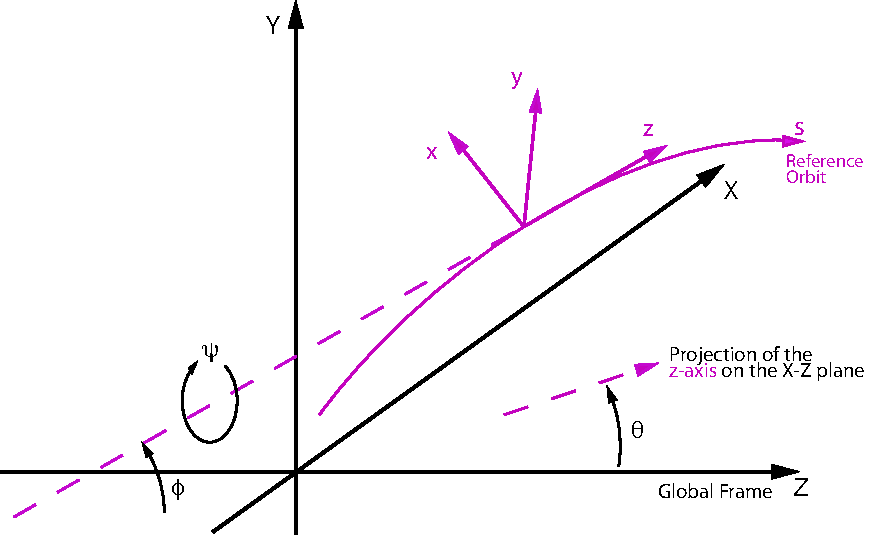
\includegraphics{floor-coords.pdf}
  \caption[The Floor Coordinate System]{
The branch coordinate system (purple), which is a function of $s$ along the branch reference
curve, is described in the floor coordinate system (black) by a position $(X(s), Y(s), Z(s))$ and
and by angles $\theta(s)$, $\phi(s)$, and $\psi(s)$.
  }
  \label{f:floor.coords}
\end{figure}

The Cartesian \vn{floor} coordinate system is the
coordinate system ``attached to the earth'' that is used to describe the branch coordinate
system. Following the \mad\ convention, the \vn{floor} coordinate axis are labeled $(X, Y,
Z)$. Conventionally, $Y$ is the ``vertical'' coordinate and $(X, Z)$ are the ``horizontal''
coordinates. To describe how the branch coordinate system is oriented within the floor coordinate
system, each point on the $s$-axis of the branch coordinate system is characterized by its $(X, Y,
Z)$ position and by three angles $\theta(s)$, $\phi(s)$, and $\psi(s)$ that describe the orientation
of the branch coordinate axes as shown in \fig{f:floor.coords}. These three angles are defined as
follows:
\begin{description}
%
\item[$\theta(s)$ Azimuth (yaw) angle:] 
Angle in the $(X, Z)$ plane between the $Z$--axis and the projection of the $z$--axis onto the $(X,
Z)$ plane. Corresponds to the \vn{y_rot} element parameter (\sref{s:offset}). A positive angle of
$\theta = \pi/2$ corresponds to the projected $z$--axis pointing in the negative $X$-direction.
%
\item[$\phi(s)$ Pitch (elevation) angle:] 
Angle between the $z$--axis and the $(X,Z)$ plane. Corresponds to the \vn{x_rot} element parameter
(\sref{s:offset}). A positive angle of $\phi = \pi/2$ corresponds to the $z$--axis pointing in the
positive $Y$ direction.
%
\item[$\psi(s)$ Roll angle:] 
Angle of the $x$--axis with respect to the line formed by the intersection of the $(X, Z)$ plane
with the $(x, y)$ plane. Corresponds to the \vn{tilt} element parameter (\sref{s:offset}). A
positive $\psi$ forms a right--handed screw with the $z$--axis.
\end{description}

By default, at $s = 0$, the reference curve's origin coincides with the $(X, Y, Z)$ origin and the
$x$, $y$, and $z$ axes correspond to the $X$, $Y$, and $Z$ axes respectively. If the lattice has no
vertical bends (the \vn{ref_tilt} parameter (\sref{s:bend}) of all bends are zero), the $y$--axis
will always be in the vertical $Y$ direction and the $x$--axis will lie in the horizontal $(X,Z)$
plane. In this case, $\theta$ decreases as one follows the reference curve when going through a
horizontal bend with a positive bending angle. This corresponds to $x$ pointing radially
outward. Without any vertical bends, the $Y$ and $y$ axes will coincide, and $\phi$ and $\psi$ will
both be zero. The \vn{beginning} statement (\sref{s:beginning}) in a lattice file can be use to
override these defaults.

Following \mad, the floor position of an element is characterized by a vector $\bfV$
\begin{equation}
  \bfV = 
  \begin{pmatrix}
    X \\ Y \\ Z 
  \end{pmatrix}
\end{equation}
The orientation of an element is described by a unitary rotation matrix $\bfW$. The column vectors
of $\bfW$ are the unit vectors spanning the branch coordinate axes in the order $(x, y, z)$. $\bfW$
can be expressed in terms of the orientation angles $\theta$, $\phi$, and $\psi$ via the formula
\begin{align}
  \bfW &= \bfR_{y}(\theta) \; \bfR_{x}(-\phi) \; \bfR_{z}(\psi) 
  \label{wwww} \\
  &= \begin{pmatrix}
    \cos\theta \cos\psi - \sin\theta \sin\phi \sin\psi & 
        -\cos\theta \sin\psi - \sin\theta \sin\phi \cos\psi & 
         \sin\theta \cos\phi \\
    \cos\phi \sin\psi & \cos\phi \cos\psi & \sin\phi \\
   -\cos\theta \sin\phi \sin\psi - \sin\theta \cos\psi & 
         \sin\theta \sin\psi - \cos\theta \sin\phi \cos\psi & 
         \cos\theta \cos\phi 
  \end{pmatrix}
  \nonumber
\end{align}
where
\begin{equation}
  \bfR_{y}(\theta) = 
  \begin{pmatrix}
    \cos\theta  & 0 & \sin\theta \\
    0           & 1 & 0          \\
    -\sin\theta & 0 & \cos\theta 
  \end{pmatrix}, \quad
  \bfR_{x}(\phi) = 
  \begin{pmatrix}
    1 & 0 & 0                \\
    0 & \cos\phi & -\sin\phi \\
    0 & \sin\phi &  \cos\phi 
  \end{pmatrix}, \quad
  \bfR_{z}(\psi) = 
  \begin{pmatrix}
    \cos\psi & -\sin\psi & 0 \\
    \sin\psi &  \cos\psi & 0 \\
    0        &  0        & 1                
  \end{pmatrix}
  \label{wtt0t}
\end{equation}
Notice that these are Tait-Bryan angles and not Euler angles.

An alternative representation of the $\bfW$ matrix (or any other rotation matrix) is to specify the
axis $\Bf u$ (normalized to 1) and angle of rotation $\beta$
\begin{equation}
  \bfW = \begin{pmatrix}
    \cos \beta + u_x^2 \left(1 - \cos \beta \right) & 
    u_x \, u_y \left(1 - \cos \beta \right) - u_z \sin \beta & 
    u_x \, u_z \left(1 - \cos \beta \right) + u_y \sin \beta \\ 
    u_y \, u_x \left(1 - \cos \beta \right) + u_z \sin \beta & 
    \cos \beta + u_y^2\left(1 - \cos \beta \right) & 
    u_y \, u_z \left(1 - \cos \beta \right) - u_x \sin \beta \\ 
    u_z \, u_x \left(1 - \cos \beta \right) - u_y \sin \beta & 
    u_z \, u_y \left(1 - \cos \beta \right) + u_x \sin \beta & 
    \cos \beta + u_z^2\left(1 - \cos \beta \right)
  \end{pmatrix}
  \label{wctux2}
\end{equation}

%-----------------------------------------------------------------------------
\subsection{Lattice Element Positioning}
\label{s:ele.pos}

\accellat, again following \mad, computes $\bfV$ and $\bfW$ by starting at the first element of the
lattice and iteratively using the equations
\begin{align}
  \bfV_i &= \bfW_{i-1} \; \bfL_i + \bfV_{i-1}, 
    \label{vwlv} \\
  \bfW_i &= \bfW_{i-1} \; \bfS_i
    \label{wws}
\end{align}
$\bfL_i$ is the displacement vector for the $i$\Th element and matrix $\bfS_i$ is the rotation of
the branch coordinate system of the exit end with respect to the entrance end. For clarity, the
subscript $i$ in the equations below will be dripped. For all elements whose reference curve through
them is a straight line, the corresponding $\bfL$ and $\bfS$ are
\begin{equation}
  \bfL = 
  \begin{pmatrix}
      0 \\ 0 \\ L
  \end{pmatrix},
  \quad
  \bfS = 
  \begin{pmatrix}
      1 & 0 & 0 \\ 
      0 & 1 & 0 \\
      0 & 0 & 1
  \end{pmatrix},
  \label{l00l}
\end{equation}
Where $L$ is the length of the element. 

%-----------------------------------------------------------------------

\begin{figure}
\centering 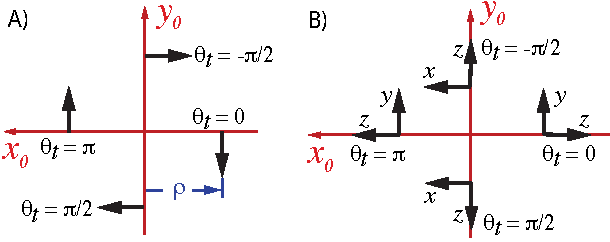
\includegraphics{tilt-bend.pdf} 
\caption[Orientation of a Bend.] 
  {
A) Rotation axes (bold arrows) for four different \vn{ref_tilt} angles of $\theta_t$ = 0, $\pm
\pi/2$, and $\pi$. $(x_0, y_0, z_0)$ are the branch coordinates at the entrance end of the bend with
the $z_0$ axis being directed into the page. Any rotation axis will be displaced by a distance of
the bend radius \vn{rho} from the origin. B) The $(x, y, z)$ coordinates at the exit end of the bend
for the same four \vn{ref_tilt} angles. In this case the bend angle is taken to be $\pi/2$.
  }
  \label{f:tilt.bend}
\end{figure}

%-----------------------------------------------------------------------

For a \vn{bend}, the axis of rotation is dependent upon the bend's \vn{ref_tilt} angle
(\sref{s:offset}) as shown in \fig{f:tilt.bend}A. The axis of rotation points in the negative $y_0$
direction for \vn{ref_tilt} = 0 and is offset by the bend radius \vn{rho}. Here $(x_0, y_0, z_0)$
are the branch coordinates at the entrance end of the bend with the $z_0$ axis being directed into
the page in the figure.  For a non-zero \vn{ref_tilt}, the rotation axis is itself rotated about the
$z_0$ axis by the value of \vn{ref_tilt}. \fig{f:tilt.bend}B shows the exit coordinates for four
different values of \vn{ref_tilt} and for a bend angle \vn{angle} of $\pi/2$.  Notice that for a
bend in the horizontal $X-Z$ plane, a positive bend \vn{angle} will result in a decreasing azimuth
angle $\theta$.

For a bend, $\bfS$ is given using \Eq{wctux2} with 
\begin{align}
  \Bf u &= (-\sin\theta_t, -\cos\theta_t, 0) \CRNO
  \beta &= \alpha_b
  \label{ustt}
\end{align}
where $\theta_t$ is the \vn{ref_tilt} angle. The $\bfL$ vector for a \vn{bend} is given by 
\begin{equation}
  \bfL = \bfR_{z}(\theta_t) \; \bftilde L, \quad
  \bftilde L = 
  \begin{pmatrix}
    \rho (\cos\alpha_b - 1) \\ 0 \\ \rho \, \sin\alpha_b
  \end{pmatrix}
  \label{lrztt}
\end{equation}
where $\alpha_b$ is the bend \vn{angle} (\sref{s:bend}) and $\rho$ being the bend radius
(\vn{rho}). Notice that since $\Bf u$ is perpendicular to $z$, the curvilinear reference coordinate
system has no ``torsion''. That is, it is a Frenet-Serret coordinate system.

Note: An alternative equation for \vn{\bfS} for a bend is
 \begin{equation}
  \bfS = \bfR_{z}(\theta_t) \; \bfR_{y}(-\alpha_b) \; \bfR_{z}(-\theta_t)
  \label{srrr}
\end{equation}

The bend transformation above is so constructed that the transformation is equivalent to rotating
the branch coordinate system around an axis that is perpendicular to the plane of the bend. This
rotation axis is invariant under the bend transformation. For example, for $\theta_t = 0$ (or $\pi$)
the $y$-axis is the rotation axis and the $y$-axis of the branch coordinates before the bend will be
parallel to the $y$-axis of the branch coordinates after the bend as shown in \fig{f:tilt.bend}. That
is, a lattice with only bends with $\theta_t = 0$ or $\pi$ will lie in the horizontal plane (this
assuming that the $y$-axis starts out pointing along the $Y$-axis as it does by default).  For
$\theta_t = \pm\pi/2$, the bend axis is the $x$-axis. A value of $\theta_t = +\pi/2$ represents a
downward pointing bend.

\begin{figure}
  \centering 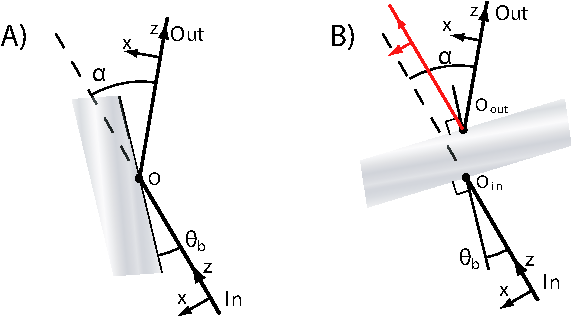
\includegraphics{mirror.pdf} 
\caption[Mirror and crystal geometry] {Mirror and crystal geometry.  The geometry shown here is
appropriate for a \vn{ref_tilt} angle of $\theta_t = 0$.  $\theta_g$ is the bend angle of the
incoming (entrance) ray, and $\alpha_b$ is the total bend angle of the reference trajectory. A)
Geometry for a mirror or a Bragg crystal. Point $\calO$ is the origin of both the branch coordinates
just before and just after the reflection/diffraction. B) Geometry for a Laue crystal.  Point
$\calO_{out}$ is the origin of the coordinates just after diffraction is displaced from the origin
$\calO_{in}$ just before diffraction due to the finite thickness of the crystal. here the bend
angles are measured with respect to the line that is in the plane of the entrance and exit
coordinates and perpendicular to the surface. For Laue diffraction, the user has the option of using
the undiffracted beam (shown in red) as the reference trajectory.
  }  
  \label{f:mirror}
\end{figure}

%-----------------------------------------------------------------------------
\subsection{Position Transformation When Transforming Coordinates}
\label{s:pos.trans}

A point $\bfQ_g = (X, Y, Z)$ defined in the floor coordinate system, when expressed in the
coordinate system defined by $(\bfV, \bfW)$ is
\begin{equation}
  \bfQ_{VW} = \bfW^{-1} \left( \bfQ_g - \bfV \right)
  \label{rwrv}
\end{equation}
This is essentially the inverse of \Eq{vwlv}. That is, position vectors propagate inversely to the
propagation of the coordinate system.

Using \Eq{rwrv} with \Eqs{vwlv}, and \eq{wws}, the transformation of a particle's position $\bfq =
(x,y,z)$ and momentum $\bfP = (P_x, P_y, P_z)$ when the coordinate frame is transformed from frame
$(\bfV_{i-1}, \bfW_{i-1})$ to frame $(\bfV_i, \bfW_i)$ is
\begin{align}
  \bfq_i &= \bfS_i^{-1} \, \left( \bfq_{i-1} - \bfL_i \right), 
    \label{rwlr} \\
  \bfP_i &= \bfS_i^{-1} \, \bfP_{i-1}
    \label{pps}
\end{align}

Notice that since $\bfS$ (and $\bfW$) is the product of orthogonal rotation matrices, $\bfS$ is
itself orthogonal and its inverse is just the transpose
\begin{equation}
  \bfS^{-1} = \bfS^T
\end{equation}

%-----------------------------------------------------------------------------
\subsection{Crystal and Mirror Entrance to Exit Coordinate Transformation}
\label{s:mirror.coords}

A \vn{crystal} element (\sref{s:mirror}) diffracts photons and a \vn{mirror} element
(\sref{s:mirror}) reflects them. For a crystal setup for Bragg diffraction, and for a mirror, the
reference curve is modeled as a zero length bend with $\bftilde L = (0, 0, 0)$, as shown in
\fig{f:mirror}A. Shown in the figure is the geometry appropriate for a \vn{ref_tilt} angle of
$\theta_t = 0$ (the rotation axis is here the $y$-axis). Since the mirror or crystal element is
modeled to be of zero length, the origin points (marked $\calO$ in the figure) of the entrance and
exit branch coordinates are the same. For Laue diffraction, the only difference is that $\bftilde L$
is non-zero due to the finite thickness of the crystal as shown in \fig{f:mirror}B. This results in
a separation between the entrance coordinate origin $\calO_{in}$ and the exit coordinate origin
$\calO_{out}$.

In all cases, the total bending angle is
\begin{align}
  \alpha_b &= \text{bragg_angle_in} + \text{bragg_angle_out} &&
                  \text{! Crystal, graze_angle_in} = 0 \CRNO
  \alpha_b &= \text{graze_angle_in} + \text{graze_angle_out} &&
                   \text{! Crystal, graze_angle_in} \ne 0 \CRNO
  \alpha_b &= 2 \, \text{graze_angle}                        &&\text{! Mirror}
  \label{agg}
\end{align}
With a mirror or Bragg diffraction, the bend angles are measured with respect to the surface
plane. With Laue diffraction the bend angles are measured with respect to the line in the bend plane
perpendicular to the surface.

For Laue diffraction, the user has the option of using the undiffracted beam (shown in red) as the
reference trajectory.

The orientation of the exit coordinates (the branch coordinates after the reflection) are only
affected by the element's \vn{ref_tilt} and bend angle parameters and is independent of all other
parameters such as the radius of curvature of the surface, etc. The branch $z$-axis of the entrance
coordinates along with the $z$-axis of the exit coordinates define a plane which is called the
element's \vn{bend plane}.  For a mirror, the graze angle is a parameter supplied by the user. For a
crystal, the Bragg angles are calculated so that the reference trajectory is in the middle of the
Darwin curve. Calculation of the Bragg angles for a crystal is given in
Section~\sref{s:crystal.ref}.

%-----------------------------------------------------------------------------
\subsection{Patch and FloorShift Entrance to Exit Transformation}
\label{s:patch.coords}

For \vn{Patch} (\sref{s:patch}) and \vn{FloorShift} (\sref{s:floor.ele}) elements, the shift in the
exit end reference coordinates is given by \Eqs{vwlv} and \eq{wws} with
\begin{align}
  \bfL &= 
    \begin{pmatrix} 
      \text{x_offset} \\ \text{y_offset} \\ \text{z_offset} 
    \end{pmatrix}
    \CRNO
  \bfS &= \bfR_{y} (\text{y_rot}) \; \bfR_{x} (\text{y_rot}) \; \bfR_{z} (\text{tilt})
  \label{swww}
\end{align}

The difference here between \vn{Patch} and \vn{SloorShift} elements is that, with a \vn{Patch}
element, the shift is relative to the exit end of the previous element while, for a \vn{FloorShift}
element, the shift is relative to the reference point on the origin element specified by the
\vn{origin_ele} parameter of the \vn{FloorShift}.

%-----------------------------------------------------------------------------
\subsection{Reflection Patch}
\label{s:reflect.patch}

A \vn{Patch} (or a series of patches) that reflects the direction of the \vn{z}-axis is called a
\vn{reflection} \vn{Patch}. By ``reflected direction'' it is meant that the dot product $\Bf z_1
\cdot \Bf z_2$ is negative where $\Bf z_1$ is the $z$-axis vector at the \vn{entrance} face and $\Bf
z_2$ is the $z$-axis vector at the \vn{exit} face. This condition is equivalent to the condition
that the associated $\bfS$ matrix (see \Eq{swww}) satisfy:
\begin{equation}
  S(3,3) < 0
  \label{s330}
\end{equation}
Using \Eq{swww} gives, after some simple algebra, this condition is equivalent to
\begin{equation}
  \cos(\text{x_rot}) \, \cos(\text{y_rot}) < 0
\end{equation}
When there are a series of patches, The transformations of all the patches are concatenated together
to form an effective $\bfS$ which can then be used with \Eq{s330}.

%-----------------------------------------------------------------------------
\subsection{Fiducial and Girder Coordinate Transformation}
\label{s:girder.coords}

For \vn{fiducial} and \vn{girder} elements, the alignment of the
reference coordinates with respect to ``\vn{origin}'' coordinates is
analogous to \Eqs{swww}. Explicitly:
\begin{align}
  \bfL &= 
    \begin{pmatrix} 
      \text{dx_origin} \\ \text{dy_origin} \\ \text{dz_origin}
    \end{pmatrix}
    \CRNO
  \bfS &= \bfR_{y} (\text{dtheta_origin}) \; \bfR_{x} (\text{-dphi_origin}) \; 
    \bfR_{z} (\text{dpsi_origin})
\end{align}

%-----------------------------------------------------------------------------
\section{Transformation Between Branch and Element Body Coordinates}
\label{s:lab.body.transform}

The \vn{element body} coordinates are the coordinate system attached to an element. Without any
alignment shifts, the \vn{branch} coordinates (\sref{s:ref}) and \vn{element body} coordinates
are the same. With alignment shifts, the transformation between \vn{branch} and \vn{element body}
coordinates depends upon whether the branch coordinate system is straight (\sref{s:straight.mis}) or
bent (\sref{s:bend.mis}).

When tracking a particle through an element, the particle starts at the \vn{nominal}
(\sref{s:coords}) upstream end of the element with the particle's position expressed in branch
coordinates. Tracking from the the nominal upstream end to the actual upstream face of the element
involves first transforming to element body coordinates (with $s = 0$ in the equations below) and
then propagating the particle as in a field free drift space from the particle's starting position
to the actual element face. Depending upon the element's orientation, this tracking may involve
tracking backwards. Similarly, after a particle has been tracked through the physical element to the
actual downstream face, the tracking to the nominal downstream end involves transforming to
branch coordinates (using $s = L$ in the equations below) and then propagating the particle as
in a field free drift space to the nominal downstream edge.

%-----------------------------------------------------------------------------
\subsection{Straight Element Branch to Body Coordinate Transformation}
\label{s:straight.mis}

For straight line elements, given a branch coordinate frame $\Lambda_s$ with origin a distance
$s$ from the beginning of the element, alignment shifts will shift the coordinates to a new reference
frame denoted $E_s$. Since alignment shifts are defined with respect to the middle of the element, the
transformation between $\Lambda_s$ and $E_s$ is a three step process:
\begin{equation}
  \Lambda_s \longrightarrow \Lambda_\text{mid} 
  \longrightarrow E_\text{mid} \longrightarrow E_s
  \label{llee}
\end{equation}
where $\Lambda_\text{mid}$ and $E_\text{mid}$ are the branch and element reference frames at the
center of the element.

The first and last transformations from $\Lambda_s$ to $\Lambda_\text{mid}$ and from $E_\text{mid}$
to $E_s$ use \Eqs{vwlv}, \eq{wws}, and \eq{l00l} with the replacement $L \rightarrow L/2 - s$ for
the first transformation and $L \rightarrow s - L/2$ for the third transformation. The middle
transformation, by definition of the offset and rotation parameters is
\begin{align}
  \bfL &= 
    \begin{pmatrix} 
      \text{x_offset} \\ \text{y_offset} \\ \text{z_offset} 
    \end{pmatrix}
    \CRNO
  \bfS &= \bfR_{y} (\text{x_rot}) \; \bfR_{x} (\text{y_rot}) \; \bfR_{z} (\text{tilt})
  \label{swww2}
\end{align}

Notice that with this definition of how elements are shifted, the position of the center of a
non-bend shifted element depends only on the offsets, and is independent of the rotations.

%-----------------------------------------------------------------------------
\subsection{Bend Element Branch to Body Coordinate Transformation}
\label{s:bend.mis}

For \vn{Bend} elements there is a \vn{ref_tilt} as well as a \vn{tilt} parameter.
The former affects both the reference curve and
the bend position (\sref{s:bend.orient}). Furthermore, \vn{ref_tilt} is calculated with respect to
the coordinates at the beginning of the bend while \vn{tilt}, \vn{x_rot},
\vn{y_rot}, and offsets are calculated with respect to the center of the chord connecting the
ends of the bend (\sref{s:align.g}). 
The different reference frame used
for \vn{ref_tilt} versus everything else means that five transformations are needed to get from the
branch frame at point $s$ to the corresponding element body frame (see \Eq{llee}). Symbolically:
\begin{equation}
  \Lambda_s \longrightarrow \Lambda_0 \longrightarrow
  \Xi_0 \longrightarrow \Xi_\text{mid} \longrightarrow 
  \Omega_\text{c,mid} \longrightarrow \Omega_{c,0} \longrightarrow 
  \Omega_{0} \longrightarrow E_0 \longrightarrow E_s
\end{equation}

\begin{enumerate}
\item $\Lambda_s \longrightarrow \Lambda_0$ \\
In branch coordinates, transform from $\Lambda_s$, the coordinates at a
distance $s$ from the beginning of the element, to $\Lambda_0$ the branch coordinates at the 
beginning of the element. This is a
rotation around the center of curvature of the bend and is given by \Eqs{vwlv} and \eq{wws} with
\Eqs{ustt} and \eq{lrztt} with the substitution $\alpha_b \rightarrow -s/\rho$.
%
\item $\Lambda_0 \longrightarrow \Xi_0$ \\
Transform from $\Lambda_s$ to $\Xi_0$ which is the ``chord''
coordinate system obtained by rotating $\Lambda_0$ around the axis perpendicular to the bend 
plane such that the $z$ axis of $\Xi_0$ is parallel to the chord. The transformation
is given by \Eqs{vwlv} with $L = (0, 0, 0)$ and $S$ given by and \eq{wws} and \eq{ustt} with
$\alpha_b \rightarrow \alpha_b/2$
%
\item $\Xi_0 \longrightarrow \Xi_\text{mid}$ \\
In chord coordinates, translate from the beginning of the chord to the end of the chord.
The transformation is given by \Eq{l00l} with $L \rightarrow L_c/2$ and $L_c$ is the chord
length.
%
\item $\Xi_\text{mid} \longrightarrow \Omega_\text{c,mid}$ \\
Transform from chord coordinates at the center of the chord to ``shifted chord coordinates''
at the same point.
This is the same transform as used for straight elements:
\begin{align}
  \bfL &= 
    \begin{pmatrix} 
      \text{x_offset} \\ \text{y_offset} \\ \text{z_offset} 
    \end{pmatrix}
    \CRNO
  \bfS &= \bfR_{y} (\text{x_rot}) \; \bfR_{x} (\text{y_rot}) \; \bfR_{z} (\text{tilt})
  \label{swwwbend}
\end{align}
%
\item $\Omega_{c,mid} \longrightarrow \Omega_{c,0}$ \\
Transform in align shifted chord coordinates from the center of the chord back to the beginning of the
chord. This is the reverse of $\Xi_0 \longrightarrow \Xi_\text{mid}$. In this case
$L \rightarrow -L_c/2$
%
\item $\Omega_{c,0} \longrightarrow \Omega_{0}$ \\
Rotate from aligned shifted chord coordinates at the entrance end to coordinates 
so that the $z$-axis is parallel to the body coordinates (tangent to the arc). 
This is the reverse of $\Lambda_0 \longrightarrow \Xi_0$. In this case $\alpha_b \rightarrow -\alpha_b/2$
%
\item $\Omega_{0} \longrightarrow E_0$ \\
Tilt (rotate around the $z$-axis) by an amount \vn{ref_tilt} which brings the coordinate system to
correspond to body coordinates at the entrance of the element.
\begin{equation}
  \bfL = 0, \quad
  \bfS = \bfR_{z}(\theta_t)
  \label{l0sr}
\end{equation}
%
\item $E_0 \longrightarrow E_s$ \\
Rotate around the
center of the bend. \Eqs{ustt} and \eq{lrztt} are used with the substitutions
$\theta_t \rightarrow 0$ and $\alpha_b \rightarrow L/\rho$.
%
\end{enumerate}
